\section{Experimenteller Aufbau und Duchführung}
\subsection{Aufbau}
Das verwendete Messgerät ist ein D8-Diffraktometer der Firma Bruker-AXS. Genutzt wird eine Kupferanode zur Erzeugung von Röntgenstrahlung.
Die zu untersuchende Probe ist ein Polystyrolfilm, der auf einem Siliziumwafer ($\SI{2}{cm}\times\SI{2}{cm}$) aufgebracht wurde. Die Röntgenröhre emittiert elektromagnetische Strahlung mit einer Wellenlänge von $\lambda=\SI{1,54}{\AA}$.
Mittels eines Göbelspiegels aus mehreren parabolisch gekrümmten Schichten wird die Strahlung zu einem parallelen Strahl gebündelt.
Danach wird die Strahlintensität durch einen Autoabsorber abgeschwächt und durch eine Blende geschickt, sodass die Streustrahlung abgedeckt ist. Die Röntgenröhre und der Detektor sind um den Probentisch über eine Software drehbar gelagert.
\subsection{Justierung}
Die Probe soll so positioniert werden, dass die Strahlung parallel zur untersuchenden Oberfläche auftrifft und die Hälfte der Intensität blockiert ist. Darüberhinaus soll auch die Probe zentriert zwischen Röntgenstrahl und Detektor ausgerichtet sein. Somit soll gewährleistet sein, dass bei einer Drehung der Probe der gesamte Strahl auf der Probenoberfläche ankommt und reflektiert wird.\\

\textbf{Detektor-Scan}:
Zu Anfang wird der Winkel der Röntgenröhre auf 0\textdegree\,gestellt und die Probe aus dem Strahl gefahren. Durchgeführt wird anschließend ein Detektor-Scan, bei dem der Detektor in einem kleinen Winkelbereich um die fest gestellte Röntgenröhre gefahren wird. Hierbei wird ein Intensitätsmaximum gemessen, das als Nullpunkt des Detektors gesetzt wird. Hiernach sollten Detektor und Strahlverlauf genau in einer Linie stehen.\\

\textbf{Z-Scan}:
Mit einem weiteren Justierungsschritt wird die Höhe der Probe in der z-Koordinate langsam erhöht. Durch das Eindringen der Probe in den Strahl sinkt die gemessene Intensität. Herausgefunden werden soll hierdurch, bei welchem Wert der z-Koordinate nur noch die halbe Intensität gemessen wird. Weitere Justierungsiterationen können nötig sein, sodass der Strahl auch wirklich parallel zur Oberfläche verläuft.\\

\textbf{Rocking-Scan}:
Bei einem Rocking-Scan werden die Röntgenröhre und der Detektor um die Probe bewegt, wobei hierbei der Winkel zwischen ihnen konstant bleiben soll. Bei diesem Vorgang wird die Intensität gemessen und der Winkel notiert, bei dem gerade keine Intensität mehr von dem Detektor gemessen werden kann. Dieser Winkel ist bei optimaler Justierung der Geometriewinkel $\alpha_G$.\\

Die jeweilig genannten Scan-Methoden sind schematisch in Abbildung \ref{scan} zu sehen.

\begin{figure}[htbp]
\begin{minipage}[c]{0.45\textwidth}
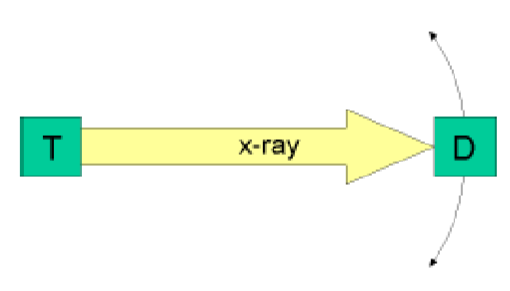
\includegraphics[width=0.78\textwidth]{bilder/detektor.png}
\centering{a)}
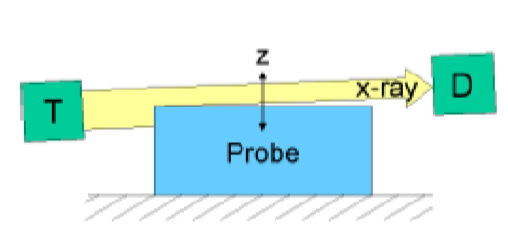
\includegraphics[width=0.78\textwidth]{bilder/zscan.png}
\centering{b)}
\end{minipage}
\begin{minipage}[c]{0.45\textwidth}
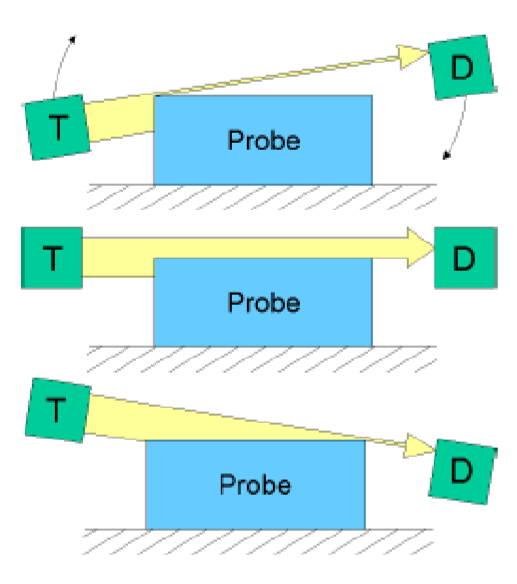
\includegraphics[width=0.78\textwidth]{bilder/rocking.png}
\centering{c)}
\end{minipage}
\caption{Schematische Darstellung. a) Detektor-Scan, b) Z-Scan und c) Rocking-Scan \cite{anleitung}.}
\label{scan}
\end{figure}

\section{Messungen}
\textbf{Reflektivitätsscan}\\
Zuerst wird ein Reflektivitätsscan durchgeführt. Hierbei werden der Einfallswinkel $\alpha_i$ zwischen Röntgenröhre und Probe und der Winkel $\alpha_r$ zwischen Probe und Detektor gleich gehalten. In einem Winkelbereich von 0\textdegree\, und 2,5\textdegree\, in 0,005\textdegree\, Schritten werden diese Winkel bewegt und jeweils für 10 Sekunden gemessen.\\

\textbf{Diffuser Scan}\\
Bei dem diffusen Scan wird der Detektorwinkel gegenüber dem Einfallswinkel um 0,1\textdegree\, verstellt, um den Anteil der gestreuten Intensität an der Reflektivität zu bestimmen. Dieser Scan kann von dem Reflektivitätsscan abgezogen werden, um die reale Reflektivität zu erhalten.
